\chapter{Referencial Teórico}

\section{A linguagem como fenômeno dialógico}
A linguagem só faz sentido quando entendemos o enunciado como resultado de uma interação social: cada fala integra respostas a vozes anteriores e abre caminho para novas respostas. Bakhtin e Faraco mostram que, ao deslocar o foco da língua como sistema para o ato concreto de falar, revelamos a dimensão histórica, ideológica e valorizacional presente em todo enunciado \cite{faraco2009, bakhtin1997estetica}. No Brasil, a multiplicidade de dialetos — identificada pelo ALiB \cite{cardoso2014alib} e detalhada por Pagani \cite{pagani2022} — reflete trajetórias de migração, práticas comunitárias e arranjos de poder que não podem ser reduzidos a meras variações fonéticas.

\section{Educação dialógica e comunicação libertadora}
Freire contrapõe o modelo de “educação bancária” ao diálogo horizontal, em que educador e educando criam conhecimento conjuntamente \cite{freire2005pedagogia, freire2013extensao}. Quando aplicado ao ambiente digital, esse princípio exige interfaces que escutem e ajustem-se ao repertório cultural dos usuários, sobretudo em contextos rurais, onde saberes tradicionais são frequentemente marginalizados. Nesse sentido, a ATER Digital Participativa propõe a coprodução de materiais didáticos e a escuta ativa das demandas locais \cite{parra2022ater, lopes2022}.

\section{Experiência e significação}
A experiência vivida é o ponto de partida para toda construção de sentido. Larrosa enfatiza seu caráter encarnado e singular, enquanto Clot destaca a linguagem como instrumento de elaboração dessa experiência \cite{larrosa2014, clot2007trabalho}. Em áreas rurais, práticas de trabalho, festas e narrativas orais moldam léxicos e entonações próprias, dimensão ressaltada por Lima ao analisar o discurso de trabalhadores \cite{lima2006}.

\section{Comunicação rural e ATER Digital Participativa}
A comunicação eficaz no campo exige respeito aos saberes locais, às formas de registro oral e às redes de troca de conhecimento \cite{zuin2021comunicacao}. Parra et al.\ mostram como tecnologias podem reforçar hierarquias ou promover diálogo genuíno, dependendo de seu desenho \cite{parra2021asbraer}. A Participação ativa dos agricultores na construção de conteúdos digitais garante maior apropriação e relevância das ferramentas.

\section{Sotaque, identidade e inclusão}
O sotaque traz marcas de identidade e memórias sociais, indo além de simples traços fonéticos \cite{bakhtin2021marxismo, bakhtin2006}. Sistemas de reconhecimento de voz geralmente falham diante de sotaques não hegemônicos, criando barreiras de acesso. Ao mapear variedades regionais a partir de códigos de área (DDDs), podemos orientar algoritmos para melhor reconhecer e assimilar essas vozes diversas.

\section{Heteroglossia aplicada ao campo}
A heteroglossia bakhtiniana refere-se à coexistência de múltiplas vozes e discursos num mesmo espaço social \cite{faraco2009}. No meio rural, isso inclui desde narrativas familiares até jargões técnicos da extensão. Para Freire, essa diversidade é fonte de riqueza e deve ser potencializada pelo diálogo \cite{freire2013extensao}. Tecnologias concebidas sob essa ótica não impõem um único “padrão” de fala, mas mediam e valorizam a multiplicidade.

\section{Contribuição deste trabalho}
Com base nesses fundamentos, este estudo propõe utilizar o mapa de Discagem Direta à Distância como ponto de partida para identificar perfis dialetais. A contribuição original consiste em:

\begin{enumerate}
  \item Adotar o DDD como camada inicial de mapeamento linguístico, aproveitando uma infraestrutura já conhecida pelo usuário.
  \item Integrar georreferenciamento fino para ajustar dialetos em áreas onde um mesmo DDD abrange variedades distintas.
  \item Implementar um mecanismo de aprendizado adaptativo que, a partir da interação real, refine continuamente o perfil linguístico de cada usuário.
  \item Incluir participação comunitária para que falantes validem e enriqueçam o mapeamento, alinhando-se aos princípios de diálogo e coautoria de Freire.
\end{enumerate}

Dessa forma, o autor propõe um sistema híbrido que conecta as teorias de Bakhtin e Freire à prática tecnológica, criando interfaces assistivas capazes de reconhecer e valorizar a riqueza dialetal brasileira. ```
\chapter{Metodologia}

\section{Mapeamento linguístico e escuta dos territórios}
Partimos de uma abordagem integrada, combinando:
\begin{enumerate}
  \item \textbf{Revisão documental:} estudos clássicos de Nascentes \cite{nascentes1953}, ALiB \cite{cardoso2014alib} e Pagani \cite{pagani2022}, para delimitar áreas dialetais.
  \item \textbf{Levantamento de DDDs:} extração de dados oficiais da Anatel \cite{anatel_pnb} e georreferenciamento das áreas de cobertura.
  \item \textbf{Associação inicial:} cruzamento DDD–dialeto segundo Pagani \cite{pagani2022} e Zuin \cite{zuin2021comunicacao}, resultando em uma tabela consolidada (\autoref{tab:tabela-ddd-local}).
  \item \textbf{Análise crítica:} identificação de sobreposições, lacunas e distorções entre divisões administrativas (DDDs) e zonas linguísticas naturais.
\end{enumerate}

\section{Adaptação regional por sotaques}
Para operacionalizar a adaptação em tecnologias assistivas, propomos um sistema híbrido:
\begin{itemize}
  \item \emph{Camada DDD:} identificação dialetal inicial pelo código de área.
  \item \emph{Georreferenciamento fino:} refinamento em subáreas, quando um DDD abriga vários subdialetos.
  \item \emph{Aprendizado adaptativo:} coleta de feedback direto do usuário para ajustar automaticamente o perfil linguístico.
  \item \emph{Participação comunitária:} mecanismos de coautoria, permitindo correções e enriquecimento contínuo do mapeamento.
\end{itemize}

\chapter{Resultados e Discussão}

\section{A divisão dialetal brasileira: De Nascentes ao ALiB}
O mapa original de Nascentes (1950) (\autoref{fig:mapa1950}) dividia o país em seis grandes regiões. Com base nos levantamentos do Projeto ALiB e nas teses de Pagani \cite{pagani2022}, ampliamos para 46 dialetos, mais sensíveis às dinâmicas urbanas e rurais. A \autoref{tab:tabela-ddd-local} consolida essa classificação.

\begin{figure}[ht]
  \centering
  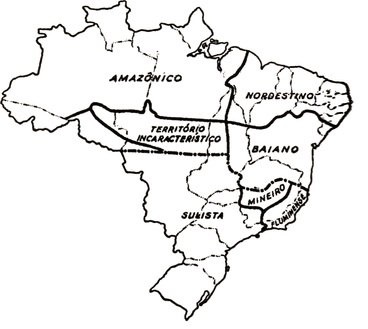
\includegraphics[width=0.75\linewidth]{images/mapa_nascentes_1950.jpeg}
  \caption{Mapa da divisão dialetal de Nascentes (1950)}
  \label{fig:mapa1950}
\end{figure}






\begin{table}[ht]
\centering
\tiny
\setlength{\tabcolsep}{6pt}
\begin{tabular}{lll}
\hline
\textbf{Dialeto} & \textbf{UF(s)} & \textbf{Área / Localização} \\
\hline
\multicolumn{3}{l}{

\textbf{Região Norte e Amazônica}} \\ \hline
Nortista    & AC, AP, AM, PA, RO, RR, TO & Interior amazônico em geral \\
Manauara    & AM                         & Manaus e entorno urbano     \\
Belenense   & PA                         & Belém e Ilha de Marajó      \\
Rondoniense & RO                         & Porto Velho e interior      \\
Paraense    & PA                         & Interior sudeste e litoral  \\
\hline
\multicolumn{3}{l}{\textbf{Região Nordeste}} \\ \hline
Nordestino (genérico) & CE, PB, PE, BA, PI & Sertão semiárido do Nordeste       \\
Cearense              & CE                  & Fortaleza e Sertão Central–Cariri  \\
Maranhense            & MA                  & São Luís e Baixada Maranhense     \\
Paraibano             & PB                  & Litoral (João Pessoa) ao Cariri    \\
Pernambucano          & PE                  & Interior agreste-sertão (exc. Recife) \\
Recifense             & PE                  & Recife e Região Metropolitana      \\
Alagoano              & AL                  & Litoral de Maceió à Zona da Mata   \\
Sergipano             & SE                  & Estado inteiro (centro em Aracaju) \\
Teresinense           & PI                  & Capital Teresina                   \\
Sertanejo             & PI, BA, PE          & Faixa sertaneja semiárida          \\
\hline
\multicolumn{3}{l}{\textbf{Região Baiana}} \\ \hline
Baiano          & BA & Interior e litoral baiano em geral      \\
Soteropolitano  & BA & Salvador e Região Metropolitana         \\
Porto-Segurense & BA & Município de Porto Seguro               \\
Caravelense     & BA & Caravelas e litoral extremo sul         \\
Paulo-Afonsino  & BA & Cidade de Paulo Afonso, norte da BA     \\
\hline
\multicolumn{3}{l}{\textbf{Região Sudeste}} \\ \hline
Mineiro           & MG                     & Zona da Mata e Sul de Minas           \\
Belo-horizontino  & MG                     & Belo Horizonte e RM                   \\
Uberlandense      & MG                     & Uberlândia e Triângulo Mineiro        \\
Campo-Belense     & MG                     & Campo Belo, sul de Minas              \\
Carioca           & RJ                     & Rio de Janeiro e Baixada Fluminense   \\
Capixaba          & ES                     & Espírito Santo (todo o estado)        \\
Vitoriense        & ES                     & Ilha de Vitória e entorno             \\
Paulistano        & SP                     & Capital São Paulo e RM                \\
Paulista (interior)& SP                    & Centro-oeste e noroeste paulista      \\
Campineiro        & SP                     & Campinas e pólo tecnológico           \\
Piracicabano      & SP                     & Eixo Piracicaba–Limeira               \\
Santista          & SP                     & Baixada Santista                      \\
Sorocabano        & SP                     & Sorocaba e região                     \\
Botucatuense      & SP                     & Botucatu e serras centrais           \\
Bragantino        & SP                     & Bragança Paulista e Circuito das Águas\\
Capão-Bonitense   & SP                     & Capão Bonito e Vale do Paranapanema   \\
\hline
\multicolumn{3}{l}{\textbf{Região Sul}} \\ \hline
Sulista      & PR, SC                & Planaltos e planalto catarinense   \\
Paranaense   & PR                    & Interior do Paraná (exc. Curitiba) \\
Curitibano   & PR                    & Curitiba e RM                      \\
Cascavelense & PR                    & Cascavel e fronteira oeste         \\
Catarinense  & SC                    & Florianópolis e interior           \\
Gaúcho       & RS                    & Todo o Rio Grande do Sul           \\
\hline
\multicolumn{3}{l}{\textbf{Região Centro-Oeste}} \\ \hline
Goiano         & GO & Eixo Anápolis–Goiânia–Rio Verde  \\
Mato-Grossense & MT & Cuiabá e centro-sul de Mato Grosso \\
Brasiliense    & DF & Brasília e cidades-satélite        \\
\hline
\end{tabular}
\caption{Dialetos brasileiros e sua localização}
\label{tab:tabela-ddd-local}
\end{table}



\section{O plano de numeração e o mapa do DDD}
O Plano de Numeração da UIT (E.164) define para o Brasil o código +55 e DDD de dois dígitos. A distribuição desigual de DDDs — com 19 no estado de SP e apenas 1 em AL — reflete critérios administrativos, não linguísticos (\autoref{fig:mapa-ddd}).

\begin{figure}[ht]
  \centering
  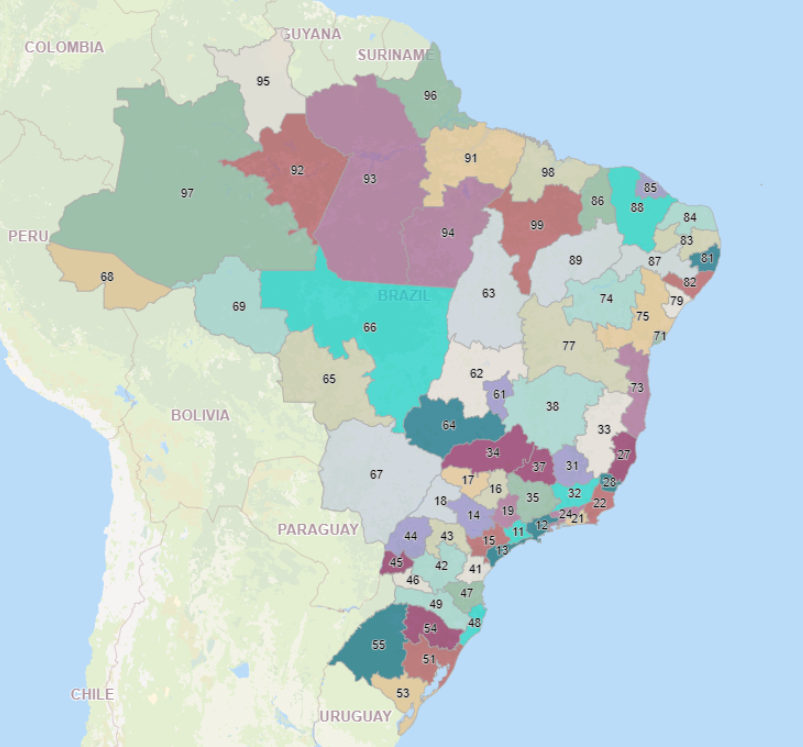
\includegraphics[width=\linewidth]{images/mapa_ddd_brasil.png}
  \caption{Mapa do Plano de Numeração Brasileiro (DDDs)}
  \label{fig:mapa-ddd}
\end{figure}

\section{Associação entre DDDs e Dialetos: Sobreposições e Lacunas}
A síntese da correspondência DDD–dialeto está em \autoref{tab:ddd-dialeto-todas}. Identificam-se:
\begin{itemize}
  \item \emph{Correspondência direta:} DDDs com dialetos quase unívocos (p.ex. 82–Alagoano, 79–Sergipano).
  \item \emph{Sobrecarga dialetal:} grandes metrópoles (11, 21) apresentam múltiplos subdialetos.
  \item \emph{Dialetos sem DDD exclusivo:} variações locais inseridas em códigos amplos (p.ex. Caravelense no 73).
\end{itemize}

\begin{table}[ht]
  \centering
  \tiny
  \setlength{\tabcolsep}{6pt}
  \begin{tabular}{llll}
    \toprule
    \textbf{DDD} & \textbf{Estados} & \textbf{Dialeto Principal} & \textbf{Subdialetos / Observações} \\
    \midrule
    \multicolumn{4}{l}{\textbf{Região Norte}} \\ 
    91 & PA      & Belenense             & Abrange a capital Belém e região metropolitana \\
    92 & AM      & Manauara              & Centrado em Manaus e entorno                  \\
    93 & PA      & Paraense              & Interior do Pará (oeste)                      \\
    94 & PA      & Paraense              & Interior do Pará (sudeste)                    \\
    95 & RR      & Nortista              & Variante roraimense                           \\
    96 & AP      & Nortista              & Variante amapaense                            \\
    97 & AM      & Nortista              & Interior do Amazonas                          \\
    98 & MA      & Maranhense            & São Luís e norte do estado                    \\
    99 & MA      & Maranhense/Nordestino & Sul do Maranhão com influências nordestinas   \\
    \midrule
    \multicolumn{4}{l}{\textbf{Região Nordeste}} \\ 
    71 & BA & Soteropolitano          & Salvador e Região Metropolitana          \\
    73 & BA & Baiano/Porto-Segurense  & Litoral sul da Bahia                     \\
    74 & BA & Baiano                  & Sertão baiano                            \\
    75 & BA & Baiano                  & Região central da Bahia                  \\
    77 & BA & Baiano/Sertanejo        & Extremo oeste baiano                     \\
    79 & SE & Sergipano               & Todo o estado de Sergipe                 \\
    81 & PE & Recifense               & Recife e Região Metropolitana            \\
    82 & AL & Alagoano                & Todo o estado de Alagoas                 \\
    83 & PB & Paraibano               & Todo o estado da Paraíba                 \\
    84 & RN & Nordestino              & Variante potiguar                        \\
    85 & CE & Cearense                & Fortaleza e região metropolitana         \\
    86 & PI & Teresinense             & Capital e centro-norte do Piauí          \\
    87 & PE & Pernambucano            & Interior de Pernambuco                   \\
    88 & CE & Cearense                & Interior do Ceará                        \\
    89 & PI & Nordestino/Sertanejo    & Sul do Piauí                             \\
    \midrule
    \multicolumn{4}{l}{\textbf{Região Centro-Oeste}} \\ 
    61 & DF/GO & Brasiliense       & Brasília, entorno e nordeste goiano   \\
    62 & GO    & Goiano            & Goiânia e centro de Goiás             \\
    63 & TO    & Nortista          & Com influências do dialeto nordestino \\
    64 & GO    & Goiano            & Sul de Goiás                          \\
    65 & MT    & Mato-Grossense    & Cuiabá e centro-sul de MT             \\
    66 & MT    & Mato-Grossense    & Norte e leste de MT                   \\
    67 & MS    & Sulista           & Com influências do dialeto paranaense \\
    68 & AC    & Nortista          & Variante acreana                      \\
    69 & RO    & Rondoniense       & Todo o estado de Rondônia             \\
    \midrule
    \multicolumn{4}{l}{\textbf{Região Sudeste}} \\ 
    11 & SP & Paulistano            & São Paulo e Região Metropolitana        \\
    12 & SP & Paulista (interior)   & Vale do Paraíba                         \\
    13 & SP & Santista              & Baixada Santista                        \\
    14 & SP & Paulista (interior)   & Bauru e região                          \\
    15 & SP & Sorocabano            & Sorocaba e região                       \\
    16 & SP & Paulista (interior)   & Ribeirão Preto e região                 \\
    17 & SP & Paulista (interior)   & São José do Rio Preto e noroeste        \\
    18 & SP & Paulista (interior)   & Presidente Prudente e oeste paulista    \\
    19 & SP & Campineiro            & Campinas e região                       \\
    21 & RJ & Carioca               & Rio de Janeiro e Região Metropolitana    \\
    22 & RJ & Fluminense            & Norte e noroeste fluminense             \\
    24 & RJ & Fluminense            & Região serrana do RJ                    \\
    27 & ES & Capixaba/Vitoriense   & Grande Vitória                          \\
    28 & ES & Capixaba              & Sul do Espírito Santo                   \\
    31 & MG & Belo-horizontino      & Belo Horizonte e Região Metropolitana    \\
    32 & MG & Mineiro               & Zona da Mata mineira                    \\
    33 & MG & Mineiro               & Vale do Jequitinhonha e Mucuri          \\
    34 & MG & Uberlandense          & Triângulo Mineiro                       \\
    35 & MG & Mineiro/Campo-Belense & Sul de Minas                            \\
    37 & MG & Mineiro               & Centro-oeste de Minas                   \\
    38 & MG & Mineiro               & Norte de Minas                          \\
    \midrule
    \multicolumn{4}{l}{\textbf{Região Sul}} \\ 
    41 & PR & Curitibano        & Curitiba e Região Metropolitana     \\
    42 & PR & Paranaense        & Centro-sul do Paraná                \\
    43 & PR & Paranaense        & Norte do Paraná                     \\
    44 & PR & Paranaense        & Noroeste do Paraná                  \\
    45 & PR & Cascavelense      & Oeste do Paraná                     \\
    46 & PR & Paranaense        & Sudoeste do Paraná                  \\
    47 & SC & Catarinense       & Norte de Santa Catarina             \\
    48 & SC & Catarinense       & Grande Florianópolis e litoral      \\
    49 & SC & Catarinense       & Oeste de Santa Catarina             \\
    51 & RS & Gaúcho            & Porto Alegre e região metropolitana \\
    53 & RS & Gaúcho            & Sul do Rio Grande do Sul            \\
    54 & RS & Gaúcho            & Serra gaúcha                        \\
    55 & RS & Gaúcho            & Oeste e noroeste do Rio Grande do Sul \\
    \bottomrule
  \end{tabular}
  \caption{Tabela de Associação DDD–Dialeto (todas as regiões)}
  \label{tab:ddd-dialeto-todas}
\end{table}

A análise dessa associação permite identificar diferentes situações:
\begin{enumerate}
    \item \textbf{Correspondência direta:} Casos em que há uma correspondência clara entre o DDD e um dialeto específico, como o DDD 71 (Salvador e Região Metropolitana) e o dialeto Soteropolitano, ou o DDD 41 (Curitiba e Região Metropolitana) e o dialeto Curitibano.
    \item \textbf{Múltiplos DDDs para um mesmo dialeto:} Situações em que um dialeto é representado por vários DDDs, como o dialeto Paulista (interior), que abrange os DDDs 12, 14, 16, 17 e 18, ou o dialeto Gaúcho, que compreende os DDDs 51, 53, 54 e 55.
    \item \textbf{DDDs que abrangem múltiplos dialetos:} Casos em que um único DDD engloba diferentes dialetos, como o DDD 73 (BA), que abrange tanto o dialeto Baiano quanto o Porto-Segurense, ou o DDD 35 (MG), que compreende tanto o dialeto Mineiro quanto o Campo-Belense.
    \item \textbf{Dialetos sem DDD específico:} Situações em que um dialeto não possui um DDD exclusivo, estando inserido em um código de área mais amplo, como o dialeto Caravelense (inserido no DDD 73), o dialeto Paulo-Afonsino (inserido no DDD 75) ou o dialeto Botucatuense (inserido no DDD 14).
\end{enumerate}

Essas sobreposições e lacunas refletem as divergências fundamentais entre os critérios de estabelecimento dos dialetos e dos DDDs. Enquanto os dialetos são formados por processos históricos, socioculturais e geográficos naturais, evoluindo organicamente ao longo de gerações, os DDDs são estabelecidos por critérios administrativos, técnicos e populacionais, seguindo estritamente divisões político-administrativas.

Além disso, a granularidade e escala dos dois sistemas são distintas. Os dialetos apresentam transições graduais e contínuas entre regiões, podendo variar significativamente dentro de um mesmo estado ou município, enquanto os DDDs possuem fronteiras rígidas e bem definidas, tendendo a agrupar grandes áreas sob um mesmo código.


Outra divergência importante refere-se à temporalidade e evolução. Os dialetos evoluem constantemente, com mudanças graduais ao longo do tempo, influenciados pela mídia e pela mobilidade populacional, enquanto o sistema de DDD é relativamente estático, com mudanças apenas por necessidades técnicas ou administrativas.


\section{Limitações e oportunidades do uso do DDD como mapa dialetetal}
A análise dos contrastes entre a divisão dialetal brasileira e o sistema de DDD revela limitações significativas, mas também oportunidades práticas para o desenvolvimento de tecnologias linguisticamente sensíveis. Entre as principais limitações, destacam-se:
\begin{enumerate}
    \item \textbf{Simplificação excessiva}: O sistema de DDD, por sua natureza administrativa, simplifica drasticamente a complexidade dialetal brasileira, agrupando áreas com significativa diversidade linguística interna sob um mesmo código.
    \item \textbf{Distorções regionais:} A distribuição dos DDDs não é uniforme pelo território nacional, com maior granularidade em regiões mais populosas e economicamente desenvolvidas, o que distorce a representação dialetal.
    \item \textbf{Fronteiras artificiais:} As fronteiras entre DDDs são definidas por limites municipais e estaduais, enquanto as fronteiras dialetais raramente coincidem com essas divisões administrativas.
    \item \textbf{Ausência de representação de microdialetos:} O sistema de DDD não captura microdialetos e variações linguísticas locais que podem ser culturalmente significativas, como as de comunidades quilombolas, indígenas e de imigrantes.
\end{enumerate}

Apesar dessas limitações, o uso do mapa de DDD como referência para o mapeamento dos dialetos brasileiros apresenta vantagens significativas:
\begin{enumerate}
    \item \textbf{Praticidade e reconhecimento:} O sistema de DDD é amplamente conhecido e utilizado pela população brasileira, facilitando a implementação de tecnologias baseadas nessa divisão.
    \item \textbf{Infraestrutura existente:} As tecnologias de telecomunicação já utilizam o sistema de DDD, o que permite a implementação imediata de soluções que considerem variações linguísticas regionais.
    \item \textbf{Correlação parcial significativa:} Apesar das divergências, existe uma correlação parcial significativa entre DDDs e dialetos, especialmente em nível macrorregional.
    \item \textbf{Escalabilidade tecnológica:} O sistema de DDD oferece uma estrutura escalável para o desenvolvimento de tecnologias adaptativas, permitindo refinamentos graduais baseados em dados de uso.
\end{enumerate}
Para superar as limitações identificadas e aproveitar as oportunidades, propomos um sistema híbrido que utiliza o DDD como primeira camada de identificação dialetal, complementada por dados georreferenciados mais precisos e pelo aprendizado adaptativo baseado na interação com o usuário. Esse sistema reconhece as áreas onde um DDD abrange múltiplos dialetos, oferecendo opções ao usuário e refinando o perfil dialetal além da identificação inicial.


\section{Implicações para tecnologias assistivas e comunicação rural}
A proposta de utilizar o mapa de DDD como referência para o mapeamento dos dialetos brasileiros tem implicações significativas para o desenvolvimento de tecnologias assistivas e para a comunicação rural. Entre as principais aplicações potenciais, destacam-se:
\begin{enumerate}
    \item \textbf{Assistentes virtuais adaptados regionalmente:} Desenvolvimento de assistentes virtuais que reconheçam e se adaptem às características linguísticas regionais, facilitando a interação com usuários de diferentes regiões do país.
    \item \textbf{Sistemas de reconhecimento de voz inclusivos:} Aprimoramento de sistemas de reconhecimento de voz para que identifiquem e processem adequadamente diferentes sotaques e variações linguísticas, reduzindo barreiras de acesso para falantes de dialetos não hegemônicos.
    \item \textbf{Interfaces de ATER Digital culturalmente sensíveis: }Criação de interfaces para serviços de Assistência Técnica e Extensão Rural Digital que se adaptem ao modo de falar local, facilitando a comunicação e o acesso a informações técnicas por parte de agricultores de diferentes regiões.
    \item \textbf{Aplicativos de tradução interdialetal:} Desenvolvimento de aplicativos que facilitem a comunicação entre falantes de diferentes dialetos, especialmente em contextos de migração interna e interação entre diferentes regiões do país.
    \item \textbf{Materiais educativos linguisticamente inclusivos}: Produção de materiais educativos digitais que respeitem e valorizem as variações linguísticas regionais, promovendo inclusão educacional e respeito à diversidade cultural.
\end{enumerate}

Essas aplicações alinham-se aos princípios do dialogismo de Bakhtin e da pedagogia libertadora de Freire, ao reconhecer e valorizar as variações linguísticas como

expressões legítimas da identidade cultural. Como destaca Freire \cite{freire2005pedagogia}, a verdadeira comunicação não se reduz à transmissão unilateral de informações, mas constitui um processo dialógico de construção compartilhada de significados, que deve respeitar e valorizar os modos de expressão locais.

No contexto específico da comunicação rural, essa abordagem ganha relevância adicional, considerando os desafios de estabelecer pontes comunicativas efetivas entre diferentes realidades socioculturais e linguísticas. Como observam Parra et al. \cite{parra2022ater}, a ATER Digital deve superar a visão instrumental da tecnologia, reconhecendo-a como mediadora de relações sociais e práticas comunicativas, que podem tanto reforçar quanto desafiar hierarquias linguísticas e sociais.













\chapter{CONCLUSÃO}
Este trabalho propôs a utilização do mapa de Discagem Direta à Distância (DDD) como referência para o mapeamento dos dialetos brasileiros, visando o desenvolvimento de tecnologias assistivas que se adaptem às variações linguísticas regionais. A análise realizada permitiu identificar correlações significativas entre os códigos de área telefônicos e os dialetos identificados no território nacional, bem como sobreposições e lacunas que refletem as divergências fundamentais entre os critérios de estabelecimento dos dois sistemas.

Os resultados revelam que, apesar das limitações, o sistema de DDD oferece uma infraestrutura prática e já estabelecida para o desenvolvimento de tecnologias que respeitem e valorizem a diversidade linguística brasileira. A proposta de um sistema híbrido, que utiliza o DDD como primeira camada de identificação dialetal, complementada por dados georreferenciados mais precisos e pelo aprendizado adaptativo, representa uma abordagem viável e escalável para superar as limitações identificadas.

As implicações dessa proposta para o desenvolvimento de tecnologias assistivas e para a comunicação rural são significativas, abrangendo desde assistentes virtuais adaptados regionalmente até interfaces de ATER Digital culturalmente sensíveis. Essas aplicações alinham-se aos princípios do dialogismo de Bakhtin e da pedagogia libertadora de Freire, ao reconhecer e valorizar as variações linguísticas como expressões legítimas da identidade cultural.

A perspectiva da teoria ator-rede de Bruno Latour também oferece insights valiosos para compreender tanto os dialetos quanto os códigos de DDD como atores em uma rede sociotécnica complexa, que influenciam e são influenciados pelas práticas comunicativas e tecnológicas. Essa abordagem permite reconhecer o potencial transformador das tecnologias linguisticamente inclusivas, que podem contribuir para

relações mais horizontais e dialógicas entre diferentes realidades socioculturais e linguísticas.

Como próximos passos para o avanço desta proposta, destacamos:

\begin{enumerate}
    \item \textbf{Desenvolvimento de protótipos:} Criação de protótipos de assistentes virtuais e sistemas de reconhecimento de voz que implementem a abordagem proposta, adaptando-se aos diferentes dialetos brasileiros com base no DDD do usuário.
    \item \textbf{Mapeamento detalhado: }Realização de um mapeamento mais detalhado e preciso das características fonéticas, prosódicas, lexicais e sintáticas de cada dialeto, associando-as aos respectivos códigos de DDD.
    \item \textbf{Testes em campo:} Realização de testes em campo com usuários de diferentes regiões do país, especialmente em contextos rurais, para avaliar a efetividade e aceitação das tecnologias desenvolvidas.
    \item \textbf{Aprimoramento contínuo:} Implementação de mecanismos de aprendizado adaptativo e feedback dos usuários, permitindo o aprimoramento contínuo do mapeamento entre DDDs e dialetos.
    \item \textbf{Expansão para outras aplicações:} Expansão da abordagem proposta para outras aplicações além de assistentes virtuais, como sistemas educacionais, serviços públicos digitais e plataformas de comunicação rural.
\end{enumerate}

Concluímos que a utilização do mapa de DDD como referência para o mapeamento dos dialetos brasileiros representa um passo significativo para o desenvolvimento de tecnologias linguisticamente inclusivas, que reconheçam e valorizem a diversidade cultural e linguística do país. Essa abordagem, fundamentada no dialogismo de Bakhtin e na pedagogia libertadora de Freire, contribui para a construção de uma sociedade digital mais inclusiva e respeitosa das diferentes formas de expressão e identidades culturais.